\newpage
\section{Подсистема справочников}

Подсистема справочников предоставляет инструменты для ведения единых справочников, которые совместно используются  \tmis и интегрируемыми подсистемами.

При переходе в подсистему справочников открывается главная страница подсистемы (Рисунок \ref{img_spr_main}).

\begin{figure}[ht]\centering
 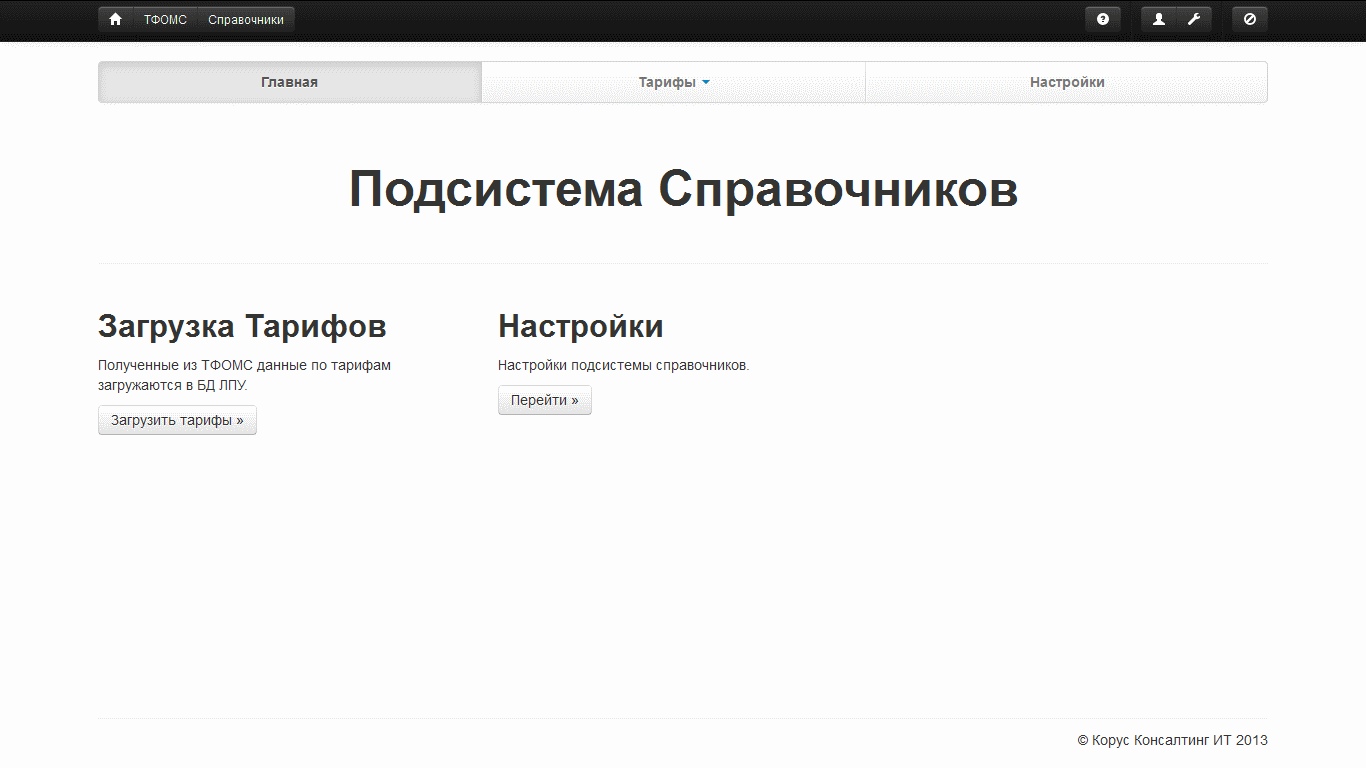
\includegraphics[width = 1\textwidth ,keepaspectratio]{spr_main}
 \caption{Главная страница подсистемы справочников}
 \label{img_spr_main}
\end{figure}

\subsection{Настройки подсистемы}

Для перехода на страницу настройки подсистемы ведения справочников нужно нажать кнопку \btn{Настройки}  в верхней части любой страницы, либо нажать кнопку  \btn{Перейти >>} в разделе \dm{Настройки} на главной странице подсистемы.

Страница настроек подсистемы имеет следующий вид (Рисунок \ref{img_spr_conf}).

\begin{figure}[ht]\centering
 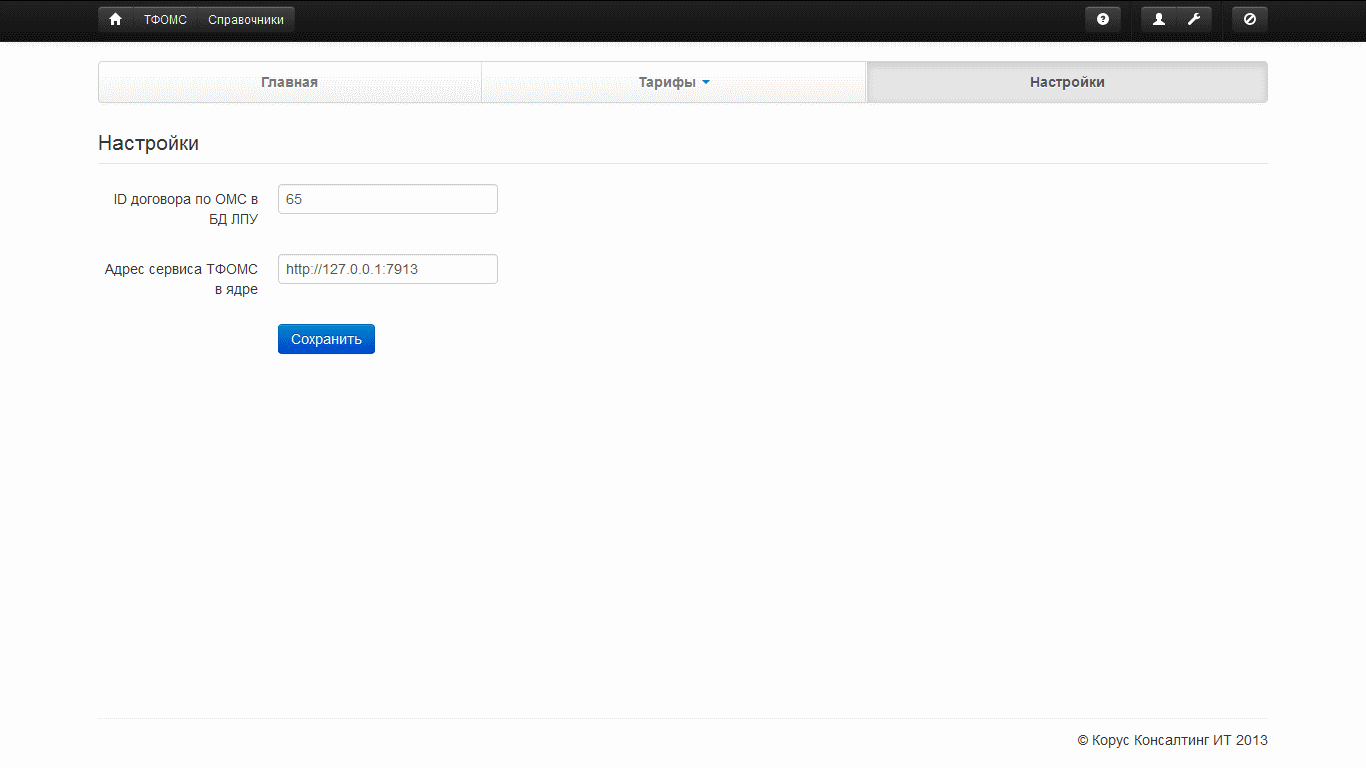
\includegraphics[width = 1\textwidth ,keepaspectratio]{spr_conf}
 \caption{Настройки подсистемы справочников}
 \label{img_spr_conf}
\end{figure}
 
